\documentclass{article}
\usepackage[utf8]{inputenc}
\usepackage{float}
\usepackage{graphicx}
\usepackage[english]{babel}
\usepackage[margin=1.7in]{geometry}
\bibliographystyle{unsrt}
\usepackage{hyperref}
\usepackage{amsmath}
\usepackage{amssymb}
\usepackage{subcaption}
\usepackage{mathtools}


\begin{document}
\begin{titlepage}
	
	
	\title{Project 2 \\ Course 02445 \\ Project in Statistical evaluation of \\ artificial intelligence }
	\author{Rasmus J. P. s164564 \\ Nikolaj S. P. s183930}
	\date{January 2020}
	\maketitle
\end{titlepage}

\section{introduction}
Briefly introduce the background \& setting of the problem, as well as the aim of the report.
Furthermore, you could give a very short description of the analysis that will be applied.

\section{Data}
The dataset consists of the yield and two measures of bioavailable phosphorous from nine fields.
With one datapoint for each plot, where each field is devided into 4 plots.
The soil was analysed for bioavailable phosphorous with two different methods "Olsen-P" and "DGT".


The yield is missing for two of the plots on field 11,
we decided to impute these two missing datapoints with the mean of the other plots from the field.
We decided on imputing instead of removing the field entirely, for two reasons.
Firstly, the fields do not have a high variance of yield between the plots, which means replacing the missing values with the mean would likely not be too far off the real values.
Secondly, field 11 is an importent datapoint with the lowest bioavailable phosphorous by far, and removing it might heavily impact our models.
 
\begin{figure}[H]
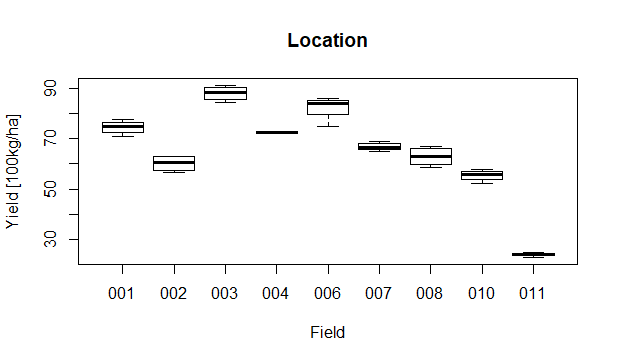
\includegraphics[width=\linewidth]{locationYield.png}
\caption{"Boxplot of yield for each field. We can see the variance within a field is relatively low, and location looks to have influence on yield"}
\label{fig:loc}
\end{figure}


Include a few good plots to highlight important features in data. You can put additional plots in the appendix.

\section{methods and analysis}

Describe the methods you used and why you decided to use them. 
Also discuss the assumptions behind the methods. Do not go into detail with theory.

\section{results}

Present the results.
Tables and figures are good ways of illustrating results.
What do your results show?
Discuss your results. How reliable are they?

\section{discussion and conclusion}

What are your conclusions? The conclusion should be connected to the aim of the report in the introduction.
	Highight important results
	
If you have found interesting problems/aspects that you haven’t carried out, you can specify them here as ‘future work’.

\end{document}